\chapter{}

%——————————————————————————————————%

\section{}






%——————————————————————————————————%

\section{}






%——————————————————————————————————%

\section{}






%——————————————————————————————————%

\section{}






%——————————————————————————————————%

\section{}






%——————————————————————————————————%

\section{}






%——————————————————————————————————%

\section{}






%——————————————————————————————————%

\section{}






%——————————————————————————————————%

\section{}






%——————————————————————————————————%

\section{}






%——————————————————————————————————%

\section{}






%——————————————————————————————————%

\section{}


图片+底部标号：
\begin{figure}[htbp]
    \centering
    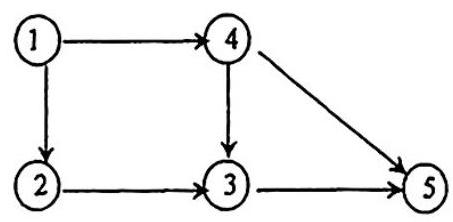
\includegraphics[width=0.3\textwidth]{images/2013/blank_17_2.jpg}
    \caption*{图2} % 使用带星号的 caption*
\end{figure}

图片+底部自动生成标号
\begin{figure}[htbp]
    \centering
    \includegraphics[width=0.3\textwidth]{你的链接}
    \caption{这里写图片的说明文字} % “图 1”会被自动加在前面
    \label{fig:my-figure}      % 这是一个标签，方便在正文中交叉引用，可选但强烈推荐
\end{figure}

代码
\begin{lstlisting}[language=C, basicstyle=\ttfamily]
% 你的代码
\end{lstlisting}

